\chapter{RELATED WORK}
\label{related}
The related works section is comprised of the more current projects being
developed in this problem domain, SDN. First an explanation of the Software
Defined Networking paradigm is presented and expounded on by the following
sections describing networking applications and the OpenFlow \cite{openflow}
specification. Next comes an overview of the different platforms and frameworks
considered during the course of this research effort. In the final topic of
this chapter the NetASM and RISC-V ISAs are discussed.

\section{Software Defined Networking}
\label{related:sdn}
SDN provides a networking device model where the control and data planes are
decoupled from one another, where a single control plane is responsible for
distributing application execution across a set of network switches viewed as
a unified data plane instance. Applications generally operate at the control
plane level and rely on distributed platforms to push the logic down to the hardware level. Allowing users to define their own control and data plane
logic enables the creation and adoption of custom networking protocols.


\section{Networking Applications}
\label{related:apps}
Not all networking applications operate in the same conceptual space, that is,
they generally act as a part of a larger system. Applications can operate on a
particular traffic flow, a node within a network, or across the entire network.
% Add more to this.

% Application pipeline figure.

\section{OpenFlow}
\label{related:of}
% Add more to this.
The OpenFlow \cite{openflow} model defines a messaging layer that the control
and, potentially distributed, data plane(s) can communicate through. This is
embodied in the OpenFlow Protocol, which specifies a set of ``instructions''
that the control and data planes must support.

\section{Heterogeneous Compute Platforms}
\label{related:hcp}
Much of the research in the domain of SDN in regards to runtime environments
encompass many of the problems found in heterogeneous computing platforms.
These issues tend to revolve around the utilization of optimized hardware
computational devices. This relates to the needs of networking programming
where a data plane is expected to be able to offload certain computation to
hardware components, such as encryption, checksums, and even packet header
processors. Below is a listing of the relevant projects in this domain that
were studied during the design and implementation of the Freeflow system.

\subsection{Heterogeneous System Architecture}
\label{related:hcp:hsa}
Or HSA \cite{hsa}, provides a specification for creating a heterogeneous
system architecture that supports the execution of applications across a 
variety of computational resources. Interfacing with these different computing 
devices requires knowledge of each devices memory model and execution 
semantics, and in order to program against them the system must provide a 
uniform view that each device conforms to.

\subsection{CUDA}
\label{related:hcp:cuda}
NVIDIA's Compute Unified Device Architecture (CUDA) \cite{cuda} for General 
Purpose Graphics Computing Units (GPGPUs) allows programmers to utilize a 
graphics card to execute applications on a SIMD device. Each graphics card 
hosts a different set of features and capabilities, such as the number of cores
available, memory architecture, and instruction sets. The CUDA library
enables developers to write a single instance of a program and deploy
it on a wide selection of supported GPUs. This is achieved by utilizing the
NVIDIA CUDA Compiler (NVCC) which translates the higher level source code
to the native device's machine code by way of an intermediate representation
(IR). The NVIDIA Virtual Machine (NVVM) IR is based on the Low Level Virtual
Machine (LLVM) IR used by the Clang compiler. Once the code has been lowered
to the NVVM IR it can be translated to the parallel thread execution virtual
machine and ISA, PTX. These instructions can be executed natively by any CUDA
enabled GPU device.

\subsection{Open Compute Language}
\label{related:hcp:ocl}
Khronos Group's Open Compute Language (OpenCL) \cite{opencl} offers an open, 
cross-platform standard for programming parallel devices. Supported devices are
personal computers, servers, and systems-on-a-chip (SOCs). The Standard
Portable IR (SPIR), based on LLVM IR, was evolved into a similarly open and 
cross-platform language called SPIR-V. This IR utilizes LLVM as the target
device, and allows for device specific code to be generated from a single
application source. OpenCL focuses on the more general problem discussed in
the previous topic, supporting a larger class of computational devices.

\section{Frameworks}
\label{related:frameworks}
Discuss the frameworks considered.

\subsection{Seastar}
\label{related:frameworks:seastar}
The Seastar project \cite{seastar}, is an open source C++ framework that
takes advantage of modern architectural designs present in many high 
performance servers.

\subsection{Libevent}
\label{related:frameworks:libevent}
Libevent \cite{libevent} exposes an API for executing function callbacks
triggered by file descriptor, signal, and timeout events.

\subsection{DPDK}
\label{related:frameworks:dpdk}
Intel's Data Plane Development Kit (DPDK) \cite{dpdk} provides a framework that
allows programmers to create highly optimized data plane applications. This
platform utilizes custom drivers that provide raw access to networking devices
and computational resources. The system is tuned to natively support Intel
brand hardware and allows users to create C applications that interface with
the runtime environment. Support for higher level applications, such as C++,
require the usage of Intel's Compiler Collection (ICC), as non-portable 
compiler directives are used throughout the framework and are not directly
supported by the GNU Compiler Collection (GCC).

\subsection{Open Data Plane}
\label{related:frameworks:odp}
The OpenDataPlane (ODP) project \cite{odp} establishes an open source API for
defining networking data plane applications. ODP provides application
portability over numerous networking architectures. Use of hardware
accelerators can be achieved without burdening the user with a required
knowledge of the capabilities and features present in an execution environment.

\section{Open Virtual Switch}
\label{related:frameworks:ovs}
Open Virtual Switch (OVS) \cite{ovs} enables the distribution of data 
plane applications over an agregation of switching devices. OVS replaces
the bridge between hypervisors running ontop of a distributed machine that
is typically provided by OS kernels. The OVS controller is capable of managing
pure software and/or hardware switchs, and supports the usage of specialized 
hardware accelerators. In Figure \ref{related:ovs_arch}, an illustration of
the OVS distributed architecture is presented.

\begin{figure}[h]
\centering
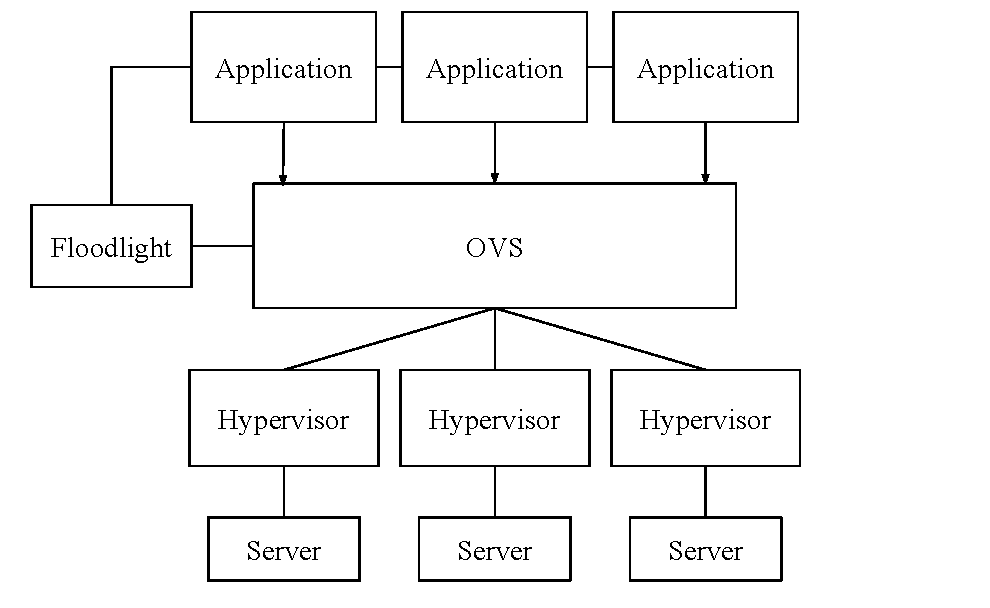
\includegraphics[scale=0.5]{ovs_arch}
\caption{The OpenVSwitch architecture.}
\label{ovs_arch}
\end{figure}

\section{NetASM}
\label{related:netasm}
The customized networking assembly language, NetASM \cite{netasm}, defines an
instruction set architecture (ISA) that tuned directly towards networking
programming. Instructions for modifying packet headers and state as well
as table and specialized operations are natively supported. In addition to the
networking oriented instructions the set also contains basic logical,
arithmetic, and control-flow operations. Applications written in NetASM can 
model the execution environment as either a traditional Turing complete 
register machine or an extended abstract machine developed by the authors.

\subsection{RISC V}
% Rewrite this.
RISC-V \cite{riscv} provides an extensible ISA, which encompasses the standard 
arithmetic, logical and control-flow operations with room for a number of user-
defined instructions.
